\section{Results: expected output, obtained output, and every graph explained}

\subsection{What we expected}
Before running the final experiments we expected:
\begin{enumerate}[label=\textbf{E\arabic*}]
  \item Correlation-aware schedulers (Kalman-greedy, the GNN) would clearly beat Max-AoI wherever sensors are
        correlated, with the same freshness guarantee.
  \item The gain would grow with correlation strength and disappear when sensors are independent.
  \item The GNN would at least match Kalman-greedy (it starts as Kalman-greedy) and beat it where looking ahead or
        robustness to a wrong model matters, especially on real data.
  \item Without the freshness guard, greedy schedulers would neglect some sensors entirely.
  \item The scheduler would be fast enough for real time: well under the 5-minute slot.
\end{enumerate}

\subsection{What we obtained (summary)}
\begin{center}
\small
\begin{tabularx}{\textwidth}{@{}lXl@{}}
\toprule
& \textbf{Obtained} & \textbf{Verdict} \\
\midrule
E1 & Synthetic: about 50\% (uniform) and 69\% (clustered) lower MSE than Max-AoI. Intel: 20\% lower RMSE. PEMS-BAY: 2.4\%. & Confirmed; much larger indoors \\
E2 & Gain $\approx$3\% at length scale 0.05, $\approx$68\% at 0.45. & Confirmed \\
E3 & GNN beats Kalman-greedy in 10/10 Intel and 15/15 PEMS-BAY windows; 73\% of synthetic layouts; ties on clustered layouts. Kalman-greedy is better on synthetic networks of 100+ sensors. & Mostly confirmed \\
E4 & Without the guard Kalman-greedy never polls 18 of 50 sensors; the GNN polls all of them. & Confirmed \\
E5 & 4.6\,ms (Intel), 37\,ms (PEMS-BAY) per slot vs.\ a 300-second slot. & Confirmed \\
\bottomrule
\end{tabularx}
\end{center}

Unexpected findings: (i) on real data, the model \emph{without message passing} matches the full GNN; (ii) on
PEMS-BAY, Kalman-greedy is \emph{worse} than plain Max-AoI because its fitted model is over-confident; (iii) the GNN
beats even the oracle that knows the true covariance on synthetic data.

\subsection{How to read the figures}
All figures use the same colours: \textbf{blue} = GNN-PPO (ours), \textbf{orange-red} = Max-AoI (B1),
\textbf{teal} = Kalman-greedy, \textbf{gold} = Corr-diverse (v4), \textbf{pink} = oracle-greedy or the ablation (dotted),
\textbf{green} = max-uncertainty, \textbf{purple} = random. Error bars and shaded bands are 95\% confidence intervals:
if two bands do not overlap, the difference is clearly real. ``Lower is better'' for every error axis.

%-------------------------------------------------------------------------------
\subsection{Figure: live scheduling on real data (the hero figure)}
\begin{figure}[H]\centering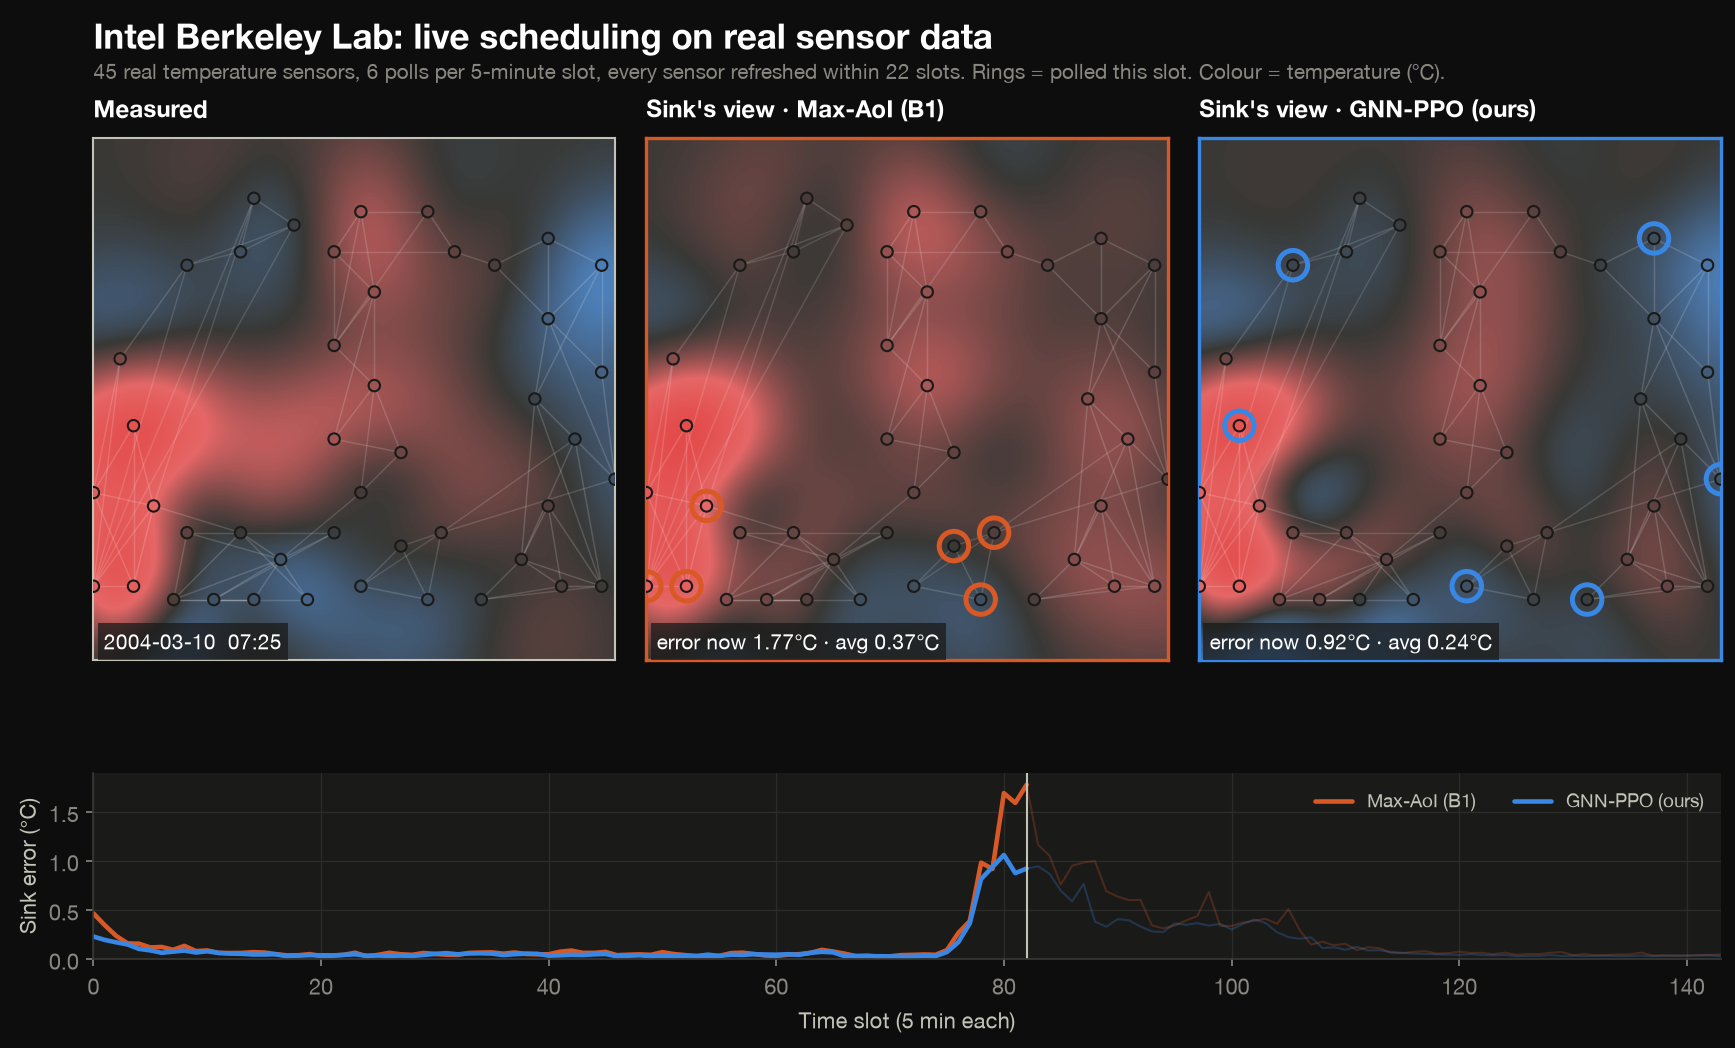
\includegraphics[width=\textwidth]{hero.png}
\caption{Intel Lab, one moment of a replay: the measured field and the sink's view under Max-AoI and under the GNN.}\end{figure}

\textbf{What is shown.} Three maps of the lab floor at 10 March 2004, 07:25. Colour is temperature (blue cool, red
warm). Left: the measured readings. Middle and right: what the sink \emph{believes} the floor looks like under
Max-AoI and under our GNN. Circles with rings are the sensors polled in this slot; thin lines are correlation-graph
edges. The bottom panel is the sink's error over 144 slots (12 hours).

\textbf{What it shows.} Around slots 75--85 the temperatures change quickly. Max-AoI's error
spikes to about 1.8\,$^\circ$C because it keeps polling sensors in fixed rotation; the GNN's spike stays near 1\,$^\circ$C because it
polls sensors spread across regions that are changing. Averages over the whole replay: 0.37\,$^\circ$C (Max-AoI) vs.\ 0.24\,$^\circ$C (GNN).

\begin{saybox}
``Left is reality, the other two are what the base station thinks. When the lab suddenly warms up, the classic
scheduler is still polling sensors in turn, so its picture goes wrong by almost 2 degrees. Our scheduler spends its
six transmissions on sensors that cover the changing areas, so its picture stays close to reality.''
\end{saybox}

%-------------------------------------------------------------------------------
\subsection{Figure: real-data benchmark (main result)}
\begin{figure}[H]\centering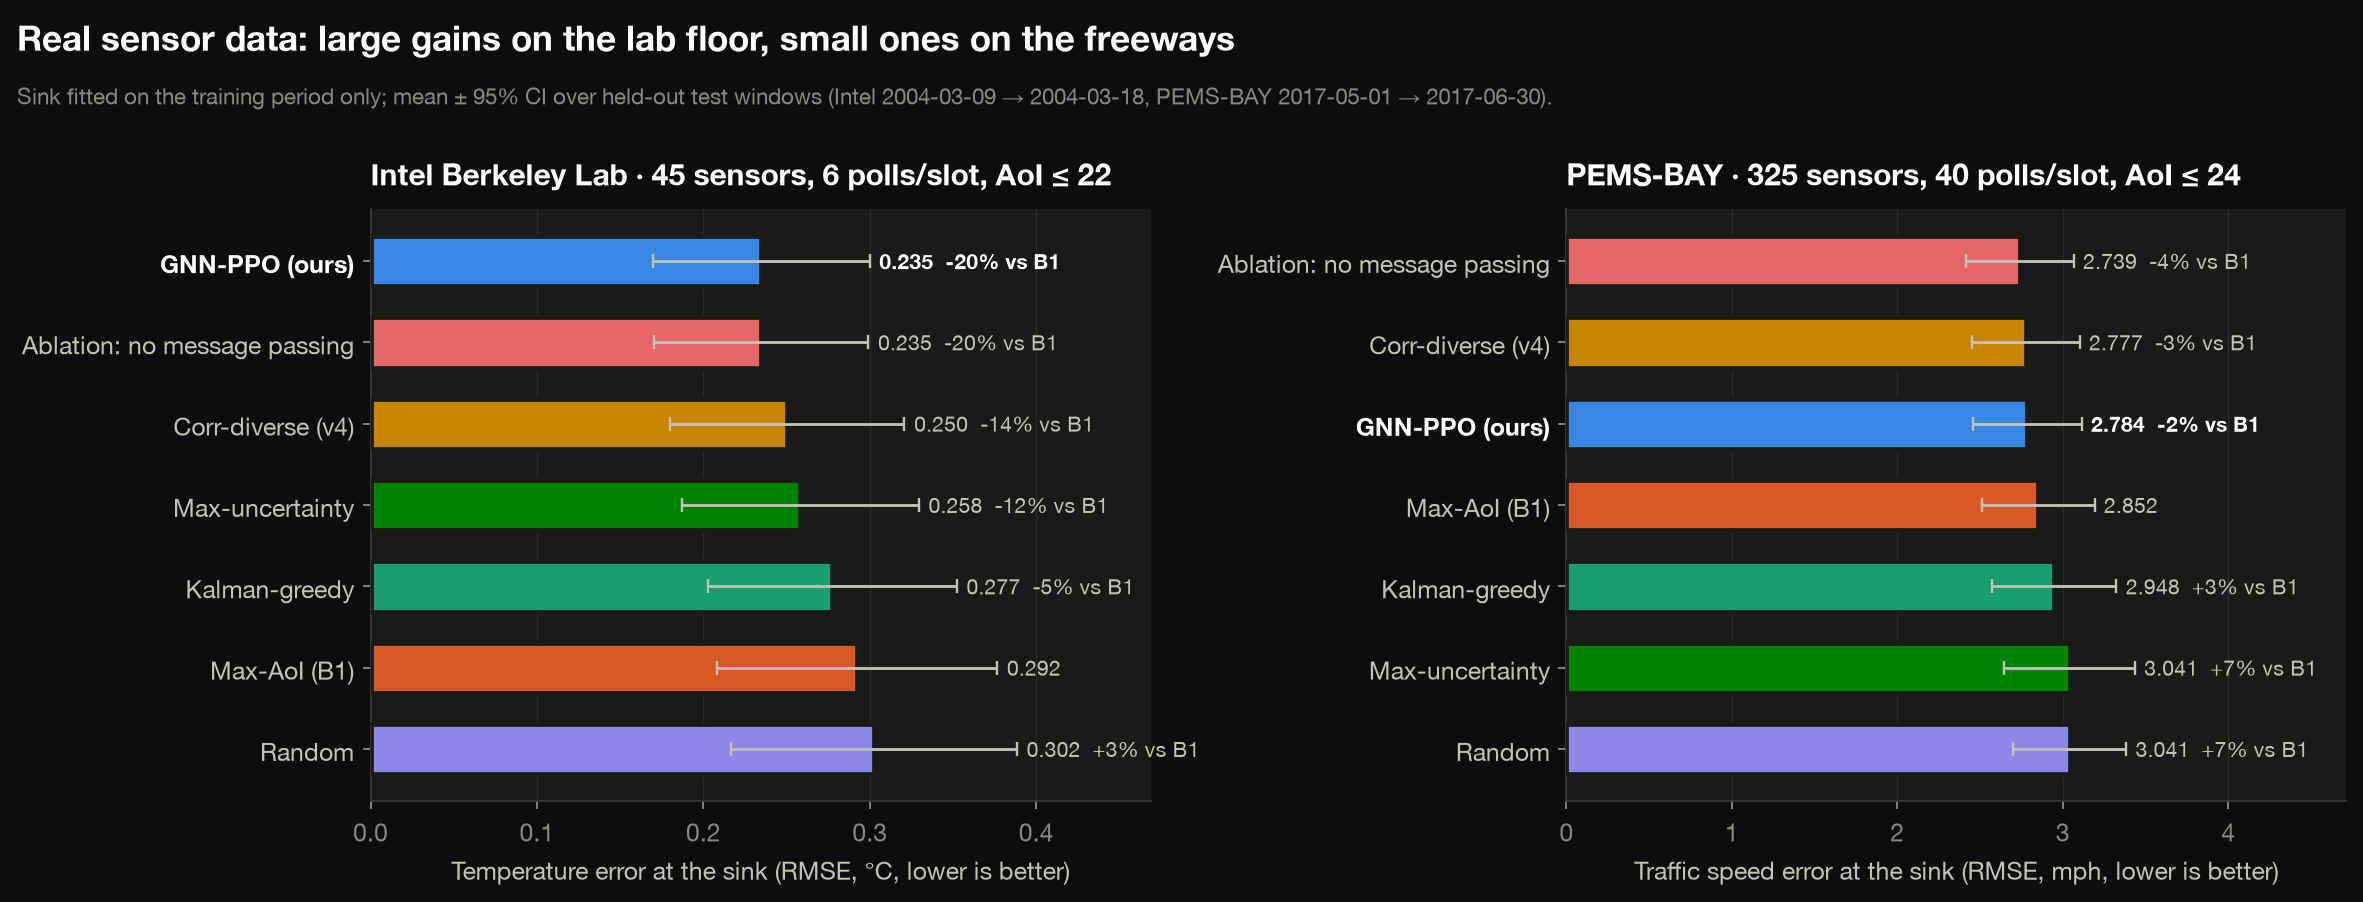
\includegraphics[width=\textwidth]{real_benchmark.png}
\caption{Sink RMSE on the held-out test periods. Left: Intel Lab (10 windows). Right: PEMS-BAY (15 windows).}\end{figure}

\begin{center}
\small
\begin{tabular}{@{}lcccc@{}}
\toprule
& \multicolumn{2}{c}{\textbf{Intel Lab} ($^\circ$C)} & \multicolumn{2}{c}{\textbf{PEMS-BAY} (mph)} \\
\textbf{Scheduler} & RMSE & mean AoI & RMSE & mean AoI \\
\midrule
Random & 0.302 & 6.72 & 3.041 & 7.27 \\
Max-AoI (B1) & 0.292 & 4.27 & 2.852 & 4.57 \\
Corr-diverse (v4) & 0.250 & 4.67 & 2.777 & 4.76 \\
Max-uncertainty & 0.258 & 5.37 & 3.041 & 6.28 \\
Kalman-greedy & 0.277 & 6.67 & 2.948 & 5.90 \\
\textbf{GNN-PPO (ours)} & \textbf{0.235} & 4.41 & \textbf{2.784} & 4.77 \\
Ablation (no message passing) & 0.235 & 4.40 & 2.739 & 4.69 \\
\bottomrule
\end{tabular}
\end{center}

\textbf{How to read it.} Each bar is a scheduler's average error over all test windows; the label shows the value and
the change against Max-AoI. Bars are sorted best at the top.

\textbf{Intel Lab.} The GNN has the lowest error, 0.235\,$^\circ$C, 20\% below Max-AoI and 15\% below Kalman-greedy. It wins
against Kalman-greedy in all 10 windows (Wilcoxon $p=0.002$) and against v4 in 8 of 10 ($p=0.05$). In standardised
MSE the GNN is 40.5\% below Max-AoI and 25.8\% below Kalman-greedy.

\textbf{PEMS-BAY.} Gains are smaller: the GNN is 2.4\% below Max-AoI in mph. Kalman-greedy is 3\% \emph{worse} than
Max-AoI: its fitted model is over-confident on traffic (it thinks it knows sensors it does not), so it neglects them.
The GNN, trained on real replays with the same kind of mismatch, does not fall into this; it beats Kalman-greedy in
15 of 15 windows ($p=6\times10^{-5}$). In standardised MSE the GNN is 10.7\% below Max-AoI and 13.4\% below
Kalman-greedy.

\begin{notebox}[Why the percentages in MSE and RMSE differ]
RMSE is the square root of MSE, which roughly halves a relative change (10\% lower MSE $\approx$ 5\% lower RMSE). And
RMSE in mph weights sensors by their natural variability: freeway sensors with large speed swings dominate, and those
are the hardest to infer from neighbours. Both numbers are correct; we report RMSE in units as the headline because it
is the error a user would see.
\end{notebox}

\begin{saybox}
``On the lab data, with the same 6 transmissions per 5 minutes and the same 2-hour freshness guarantee, our
scheduler's temperature error is 0.235 degrees against 0.292 for the classic scheduler, 20 percent lower, and it beats
the model-based greedy scheduler in every single test window. On the freeway data the improvement is smaller, 2.4
percent, because traffic sensors are less redundant, but it is still consistent: 15 out of 15 days.''
\end{saybox}

%-------------------------------------------------------------------------------
\subsection{Figure: real-data capacity and size sweeps}
\begin{figure}[H]\centering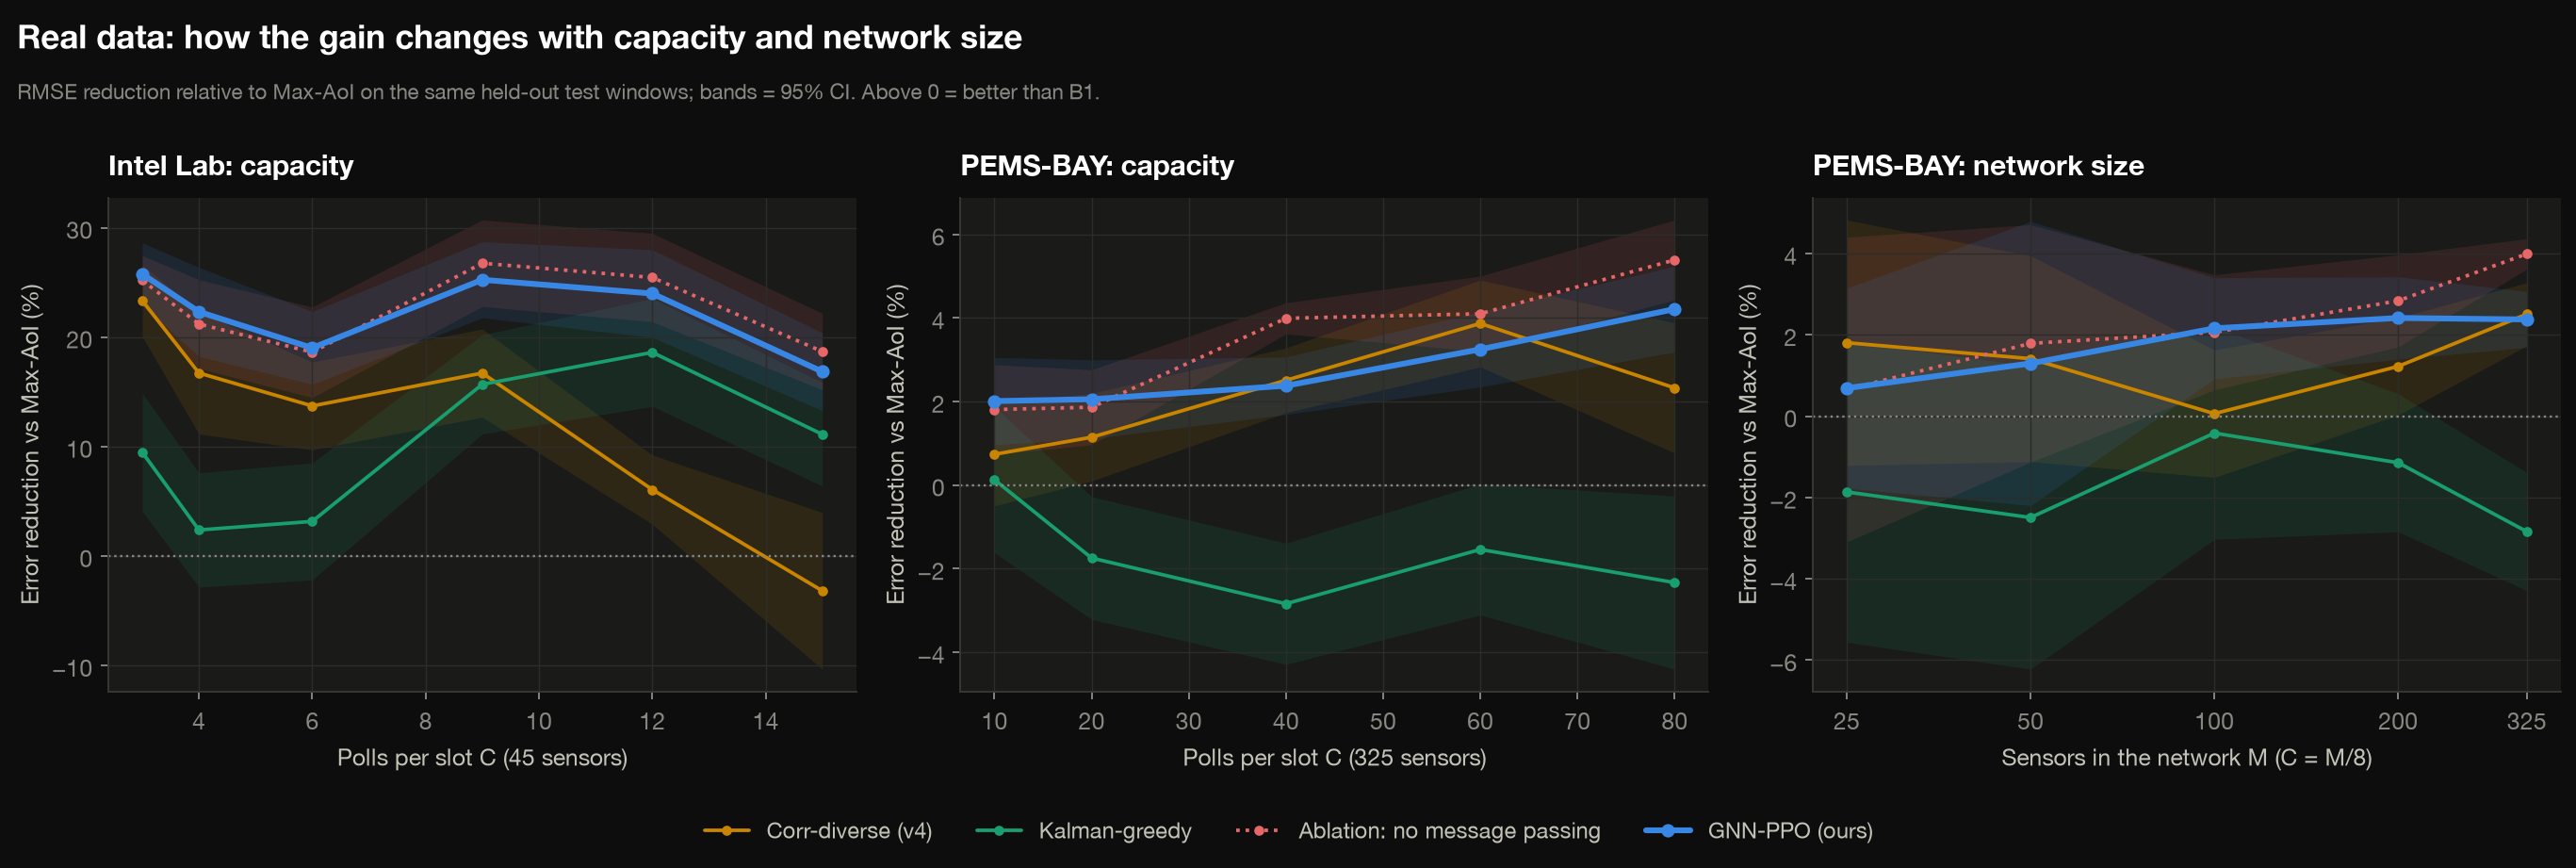
\includegraphics[width=\textwidth]{real_sweeps.png}
\caption{Error reduction against Max-AoI (above 0 = better) on real test windows, as capacity and network size vary.}\end{figure}

\textbf{How to read it.} The y-axis is ``percent less error than Max-AoI''. The dotted line at 0 means ``same as
Max-AoI''. Each line is a scheduler; the band is its 95\% CI.

\textbf{Left (Intel, capacity $C=3$ to 15).} The GNN (blue) stays 17--26\% better than Max-AoI at every capacity. The
heuristics are inconsistent: v4 drops below zero at $C=15$; Kalman-greedy ranges from 2\% to 19\%.

\textbf{Middle (PEMS-BAY, $C=10$ to 80).} The GNN's gain grows from 2\% to 4\% as capacity grows. Kalman-greedy is
below zero almost everywhere: model over-confidence again.

\textbf{Right (PEMS-BAY sub-networks of 25 to 325 sensors, $C=M/8$).} Gains are small (1--2.4\%) but positive and grow
with network size; larger networks have more neighbours to borrow information from.

\begin{saybox}
``The result is not tuned to one setting. On the lab data the gain stays between 17 and 26 percent for every channel
capacity we tried. On traffic it is small but grows with capacity and network size, while the model-based greedy
scheduler is actually worse than the classic one.''
\end{saybox}

%-------------------------------------------------------------------------------
\subsection{Figure: where each scheduler spends the channel}
\begin{figure}[H]\centering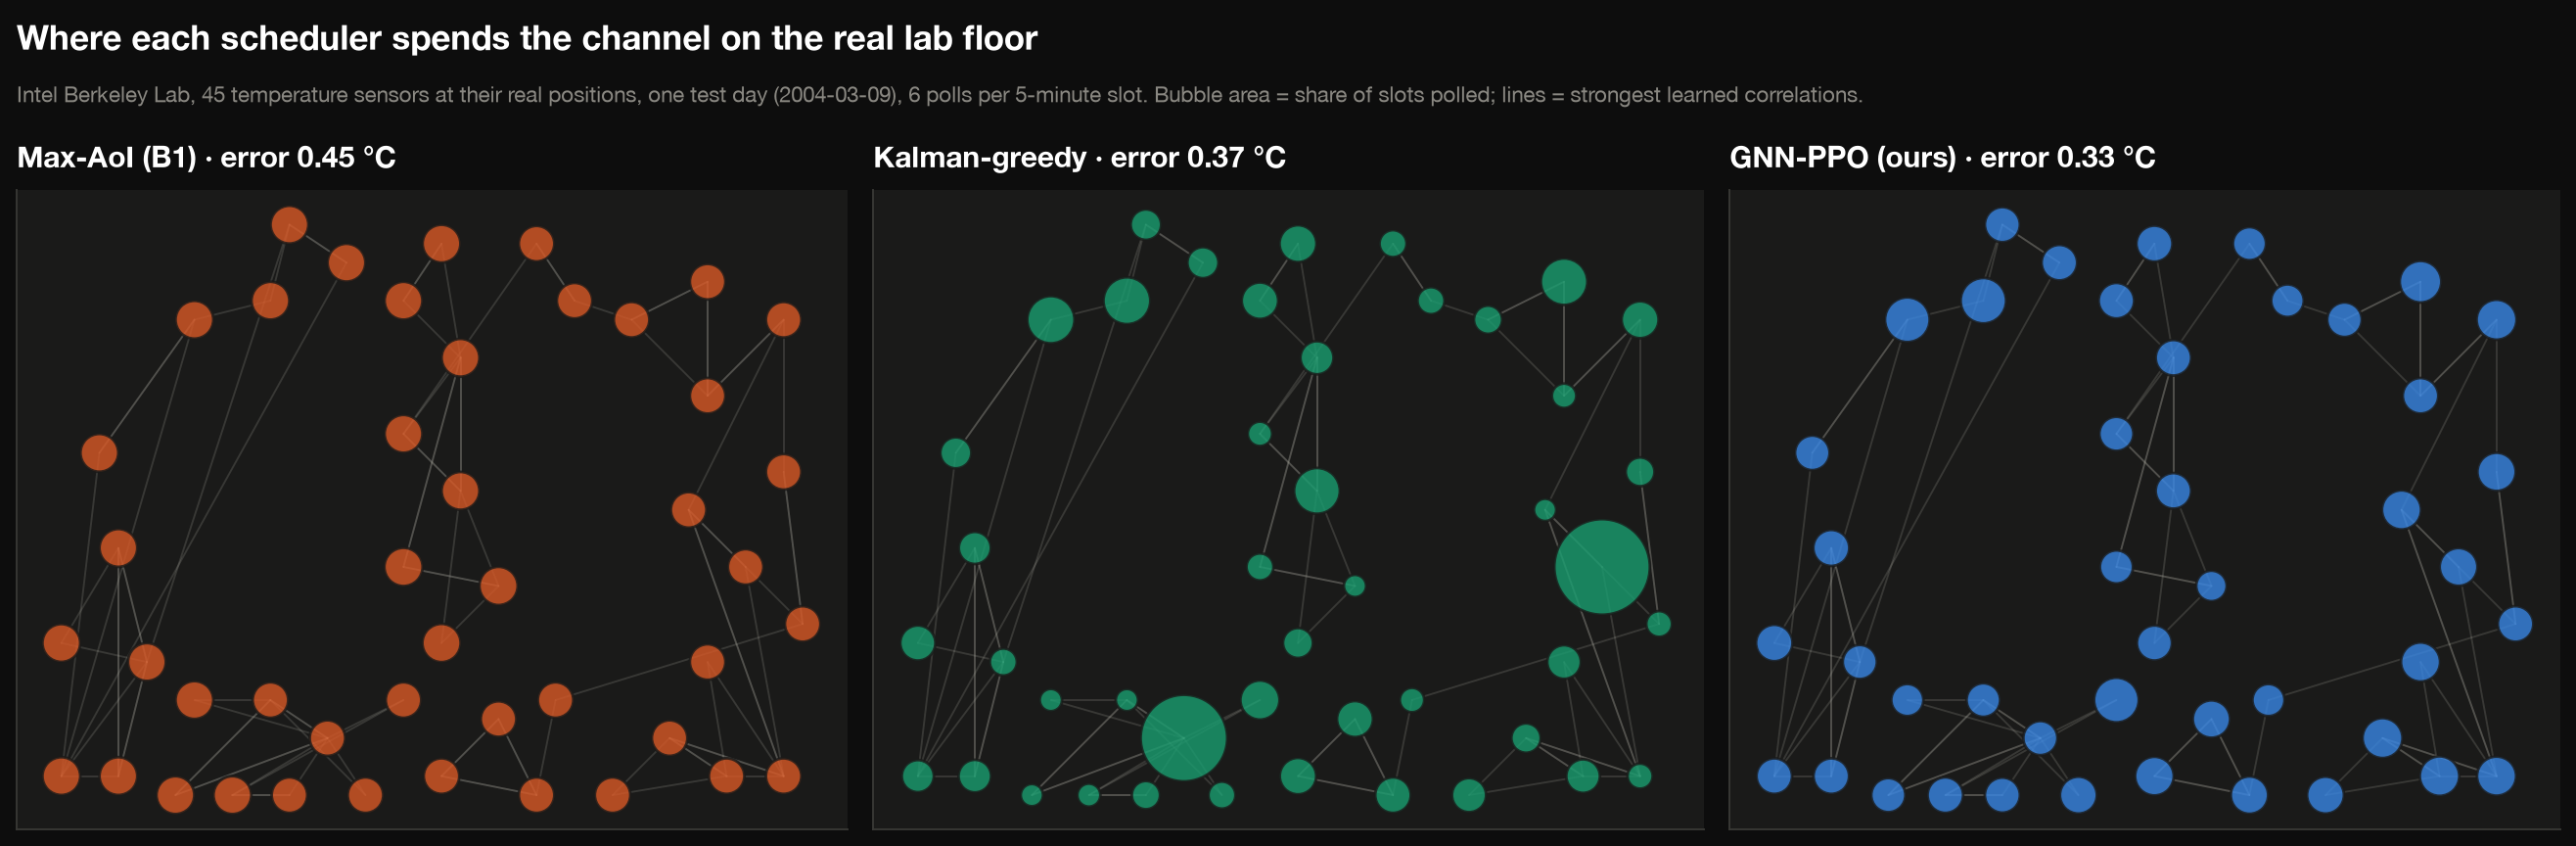
\includegraphics[width=\textwidth]{poll_map.png}
\caption{Intel Lab, one test day (9 March 2004). Bubble area = share of slots each sensor was polled.}\end{figure}

\textbf{What it shows.} Max-AoI (left) polls every sensor equally (round robin), error 0.45\,$^\circ$C. Kalman-greedy
(middle) concentrates on a few ``hub'' sensors (two huge bubbles) and polls many others only when the guard forces
it; error 0.37\,$^\circ$C. The GNN (right) spreads polls more evenly but not uniformly: more to sensors that are hard to infer,
fewer to sensors in dense, correlated groups; error 0.33\,$^\circ$C.

\begin{saybox}
``This shows \emph{how} each scheduler behaves. The classic one treats everyone equally. Greedy over-trusts its
model and fixates on a few sensors. Ours learned a balance: it polls each sensor according to how much the base
station can already guess about it.''
\end{saybox}

%-------------------------------------------------------------------------------
\subsection{Figure: synthetic benchmark}
\begin{figure}[H]\centering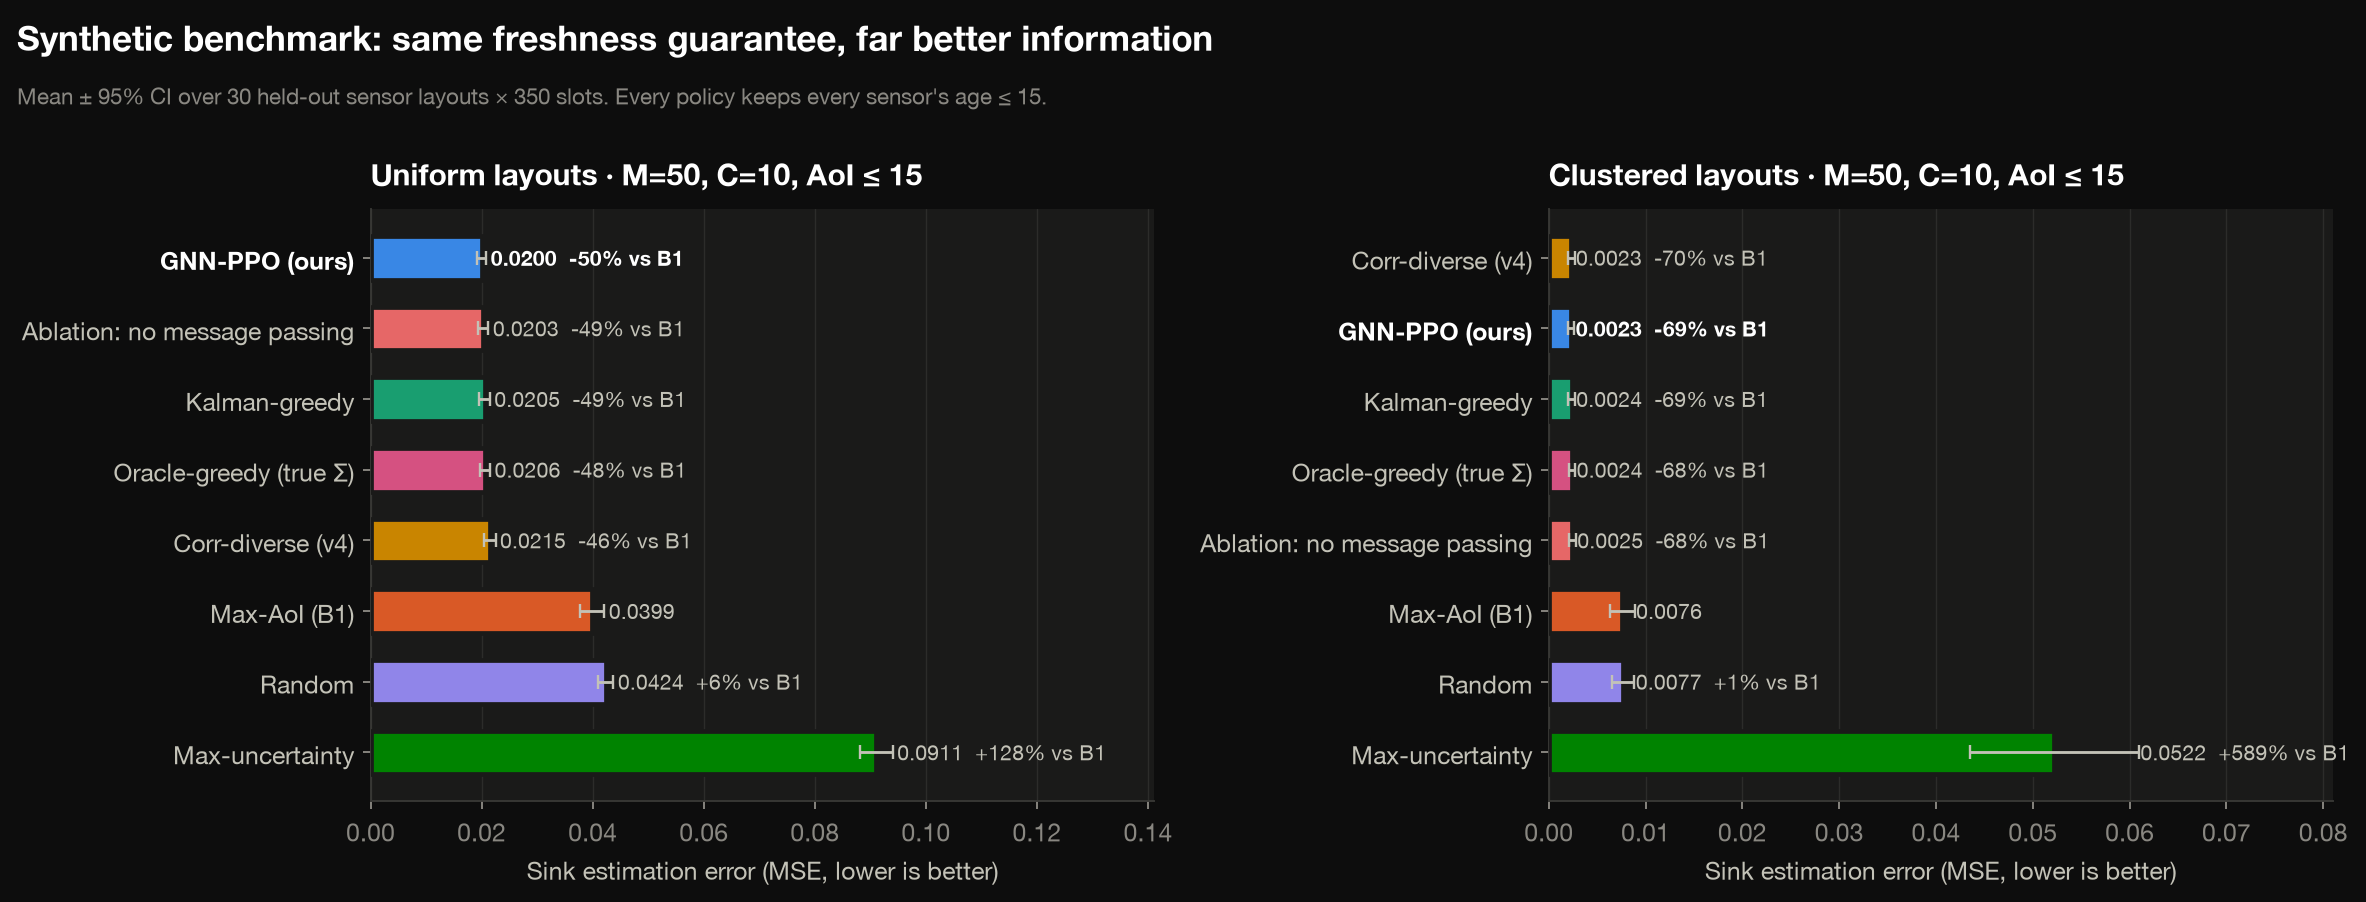
\includegraphics[width=\textwidth]{main_benchmark.png}
\caption{Synthetic fields, $M=50$, $C=10$, $F=15$, 30 unseen layouts $\times$ 350 scored slots.}\end{figure}

\textbf{Uniform layouts (left).} GNN MSE 0.0200, 50\% below Max-AoI (0.0399). It beats Kalman-greedy (0.0205) on 73\%
of layouts ($p=0.008$) and even the \emph{oracle} that knows the true covariance (0.0206) on 70\% ($p=0.003$). The
oracle is still greedy (one slot at a time); the GNN learned to look ahead. Max-uncertainty is the worst (0.0911):
polling the most uncertain sensors without considering overlap wastes polls on neighbours.

\textbf{Clustered layouts (right).} All correlation-aware schedulers reach about 0.0023--0.0024, 69\% below Max-AoI;
differences between them are not significant. In tight clusters any sensible correlation-aware rule finds the
redundancy.

\textbf{Ablation.} Removing message passing costs a little on synthetic data (GNN wins 67\% of uniform layouts and 87\%
of clustered layouts against the ablation).

\begin{saybox}
``In simulation we know the ground truth, so we can test many layouts. With the same freshness guarantee, our
scheduler halves the error of the classic scheduler, and it even beats a greedy scheduler that is given the true
correlations, because it learned to plan ahead instead of optimising one slot at a time.''
\end{saybox}

%-------------------------------------------------------------------------------
\subsection{Figure: fresher is not the same as better-informed}
\begin{figure}[H]\centering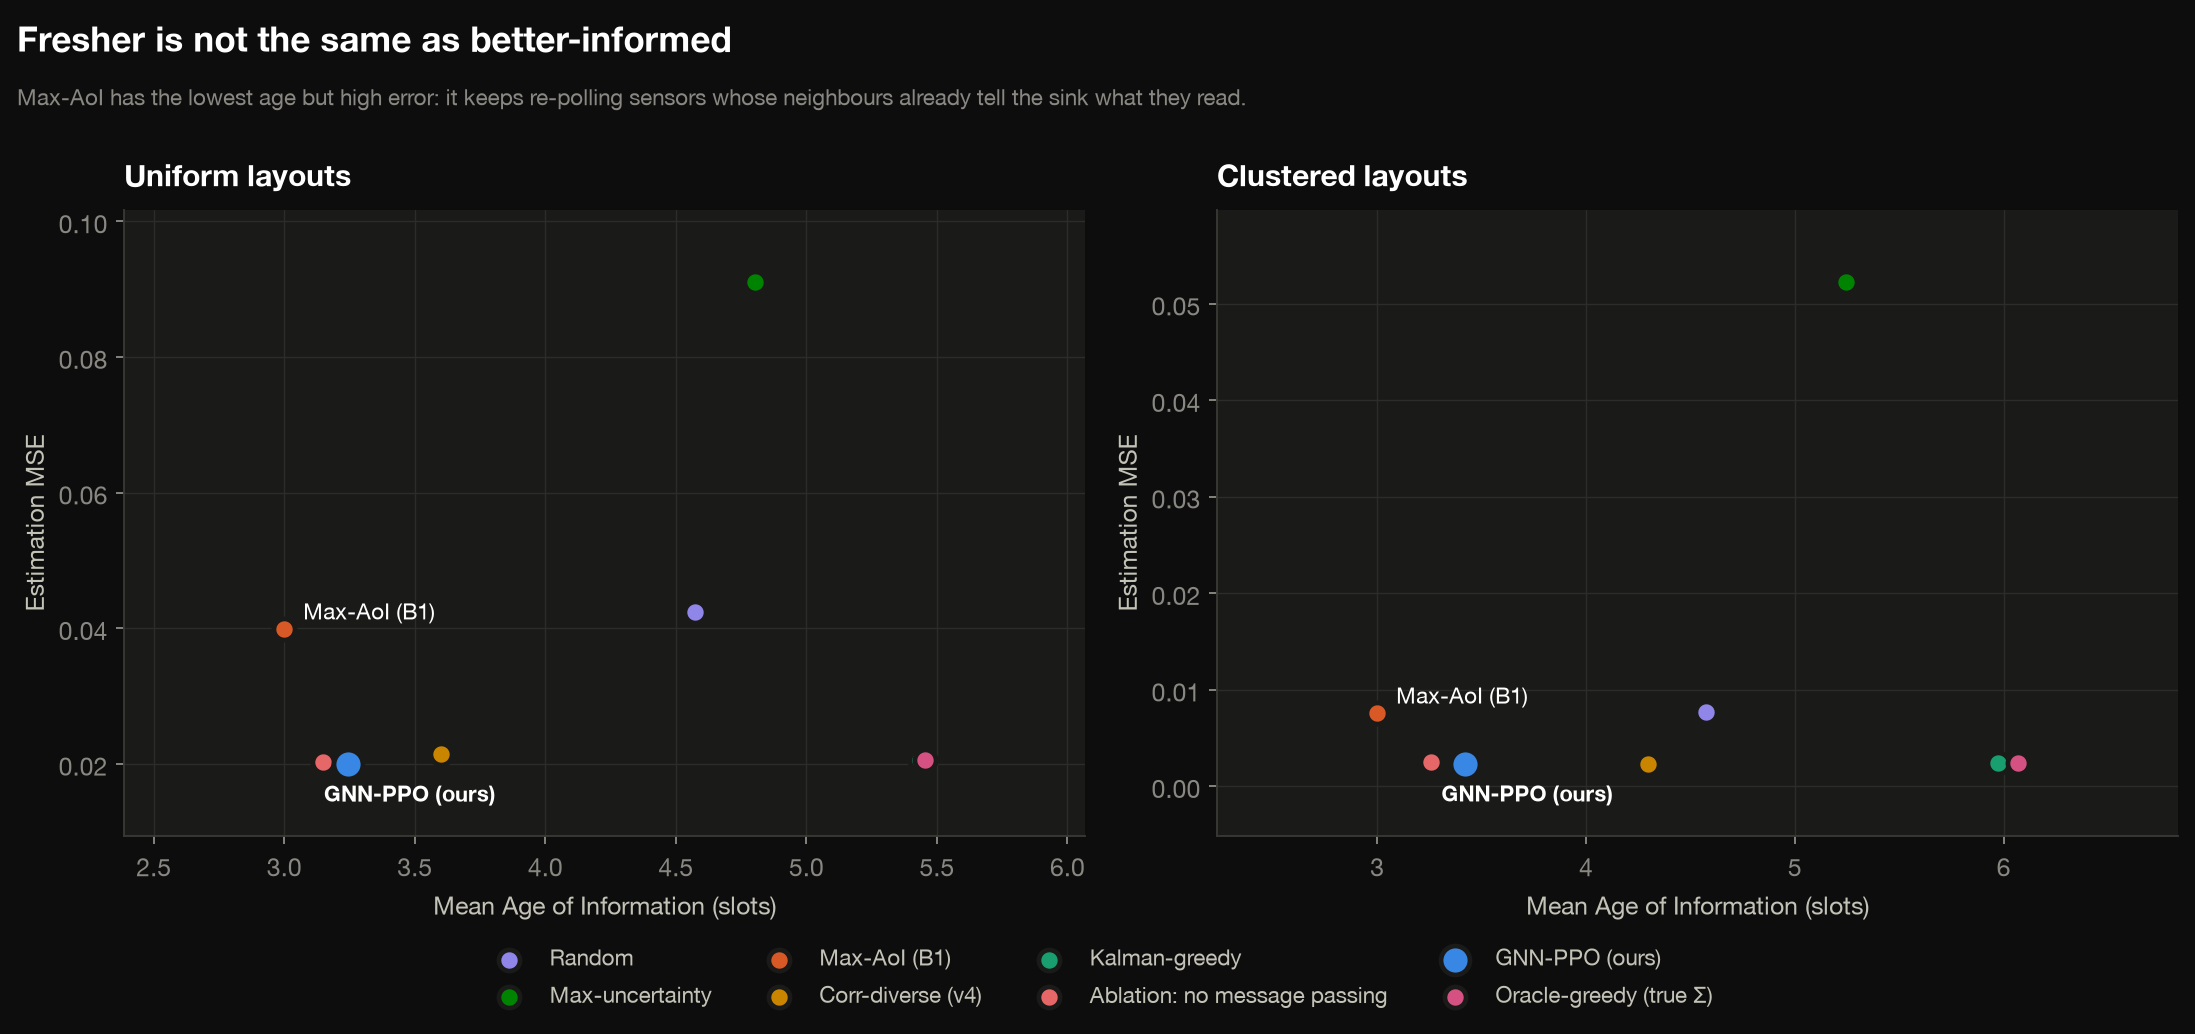
\includegraphics[width=\textwidth]{aoi_vs_error.png}
\caption{Each dot is a scheduler: mean AoI (x) against estimation error (y). Bottom-left is ideal.}\end{figure}

\textbf{What it shows.} Max-AoI has the \emph{lowest} age (3.0 slots) but about twice the error of the GNN. Kalman-greedy
and the oracle have low error but high age (5.4--6 slots): they let redundant sensors grow old. The GNN sits in the
bottom-left: low error \emph{and} low age (3.2--3.4).

\begin{saybox}
``This is the key insight of the project in one picture: minimising age is not the same as minimising error. The
classic scheduler is the freshest but not the best informed. Ours is nearly as fresh and far better informed.''
\end{saybox}

%-------------------------------------------------------------------------------
\subsection{Figure: synthetic sweeps}
\begin{figure}[H]\centering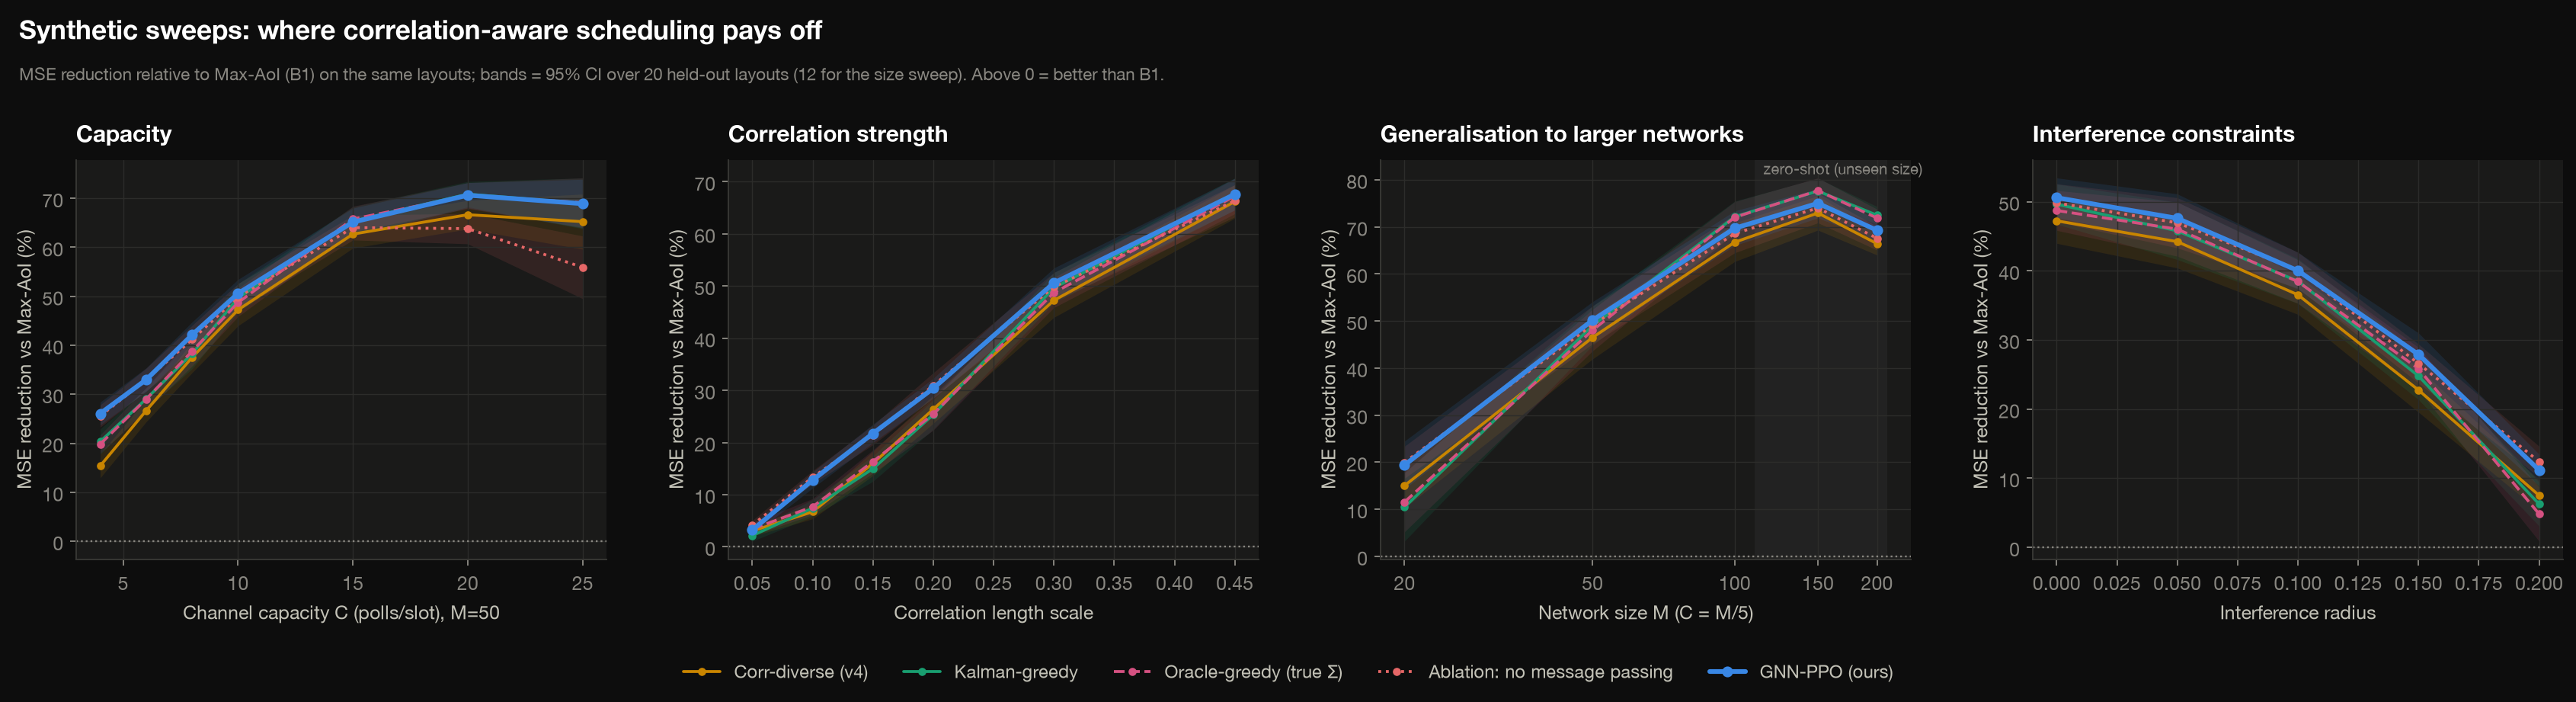
\includegraphics[width=\textwidth]{sweeps.png}
\caption{MSE reduction against Max-AoI as one setting changes at a time.}\end{figure}

\begin{itemize}
  \item \textbf{Capacity}: with very few polls ($C=4$), the GNN gains 26\% vs.\ 20\% for Kalman-greedy (GNN MSE 0.118 vs.\
        0.127): when the channel is scarce, planning matters most. The gain rises to about 70\% at $C=20$.
  \item \textbf{Correlation strength}: at length scale 0.05 (sensors almost independent) every method gains only about
        3\%: there is nothing to exploit. At 0.45 it is about 68\%. This confirms the gain really comes from
        correlation.
  \item \textbf{Network size}: training saw up to 100 sensors; 150 and 200 are \emph{zero-shot}. The GNN still gains about
        70\% vs.\ Max-AoI there, but Kalman-greedy and the oracle are 8--12\% better than the GNN for $M\ge100$.
  \item \textbf{Interference}: as more sensor pairs are forbidden to transmit together, every method's gain falls (51\%
        to 11\%) because the constraint itself forces spreading. The GNN stays at or near the top.
\end{itemize}

\begin{saybox}
``These sweeps check \emph{when} the idea works. If sensors are independent, nobody can do better than the classic
scheduler, and the curves show exactly that. The more correlated the sensors, and the scarcer the channel, the more
our approach helps.''
\end{saybox}

%-------------------------------------------------------------------------------
\subsection{Figure: how much history is needed}
\begin{figure}[H]\centering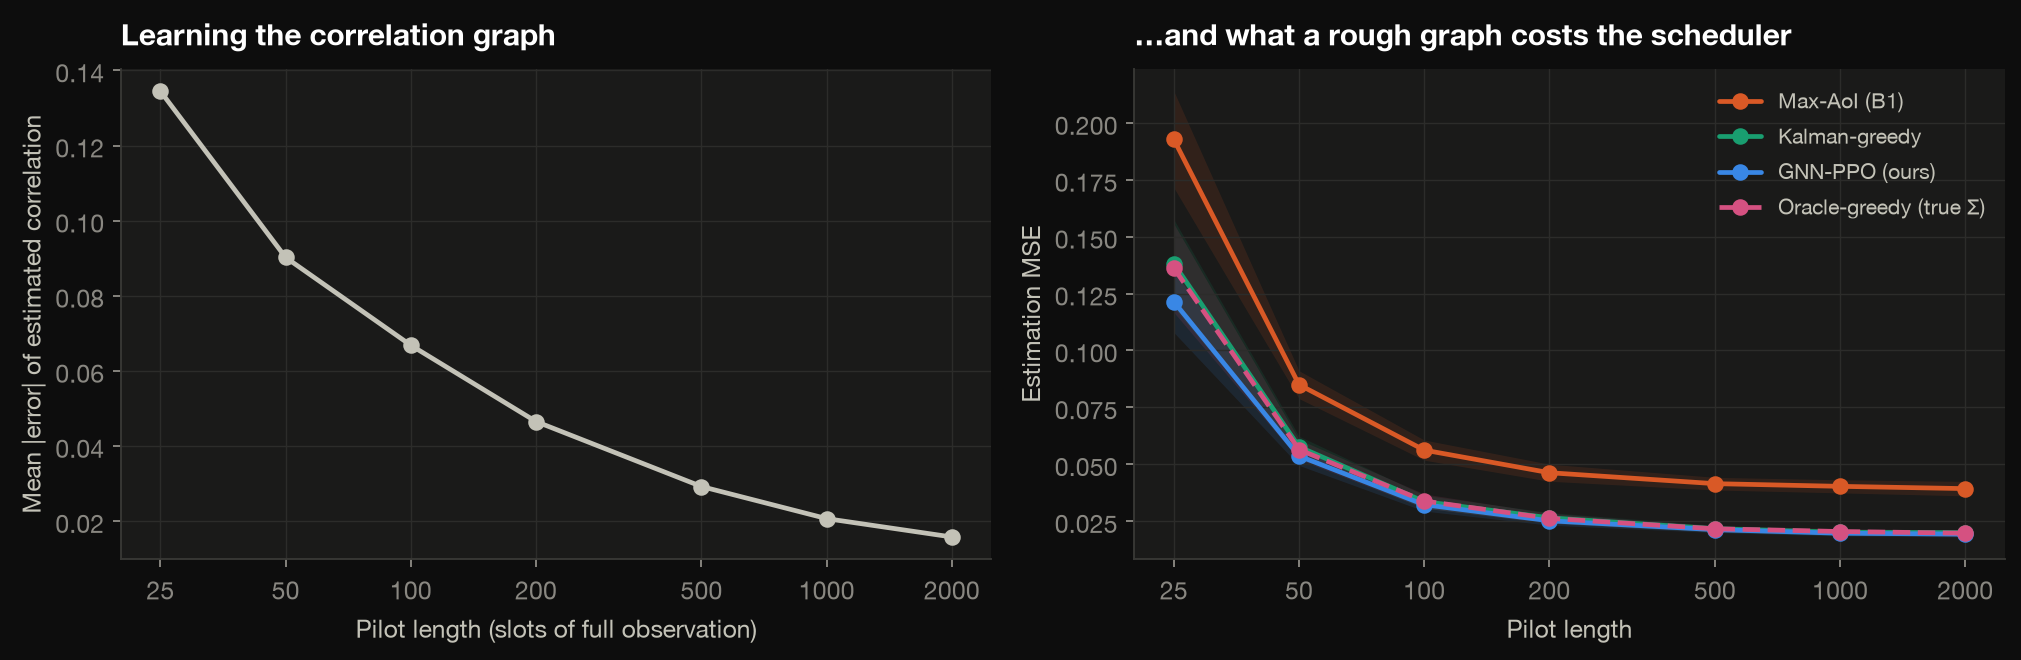
\includegraphics[width=\textwidth]{pilot_length.png}
\caption{Left: error of the learned correlations vs.\ length of the pilot (learning) phase. Right: the resulting
estimation error.}\end{figure}

\textbf{What it shows.} With only 25 slots of history the learned correlations are off by 0.135 on average; with 2000
slots, by 0.016. With rough correlations every scheduler suffers, but the GNN suffers least (MSE 0.122 vs.\ 0.138 for
Kalman-greedy at 25 slots) because it does not blindly trust the model. After about 500 slots (under two days of
5-minute data) results are close to their best.

\begin{saybox}
``How much data do we need before deploying? About 500 slots, less than two days of 5-minute readings. Even with less,
our scheduler degrades more gracefully than the model-based one.''
\end{saybox}

%-------------------------------------------------------------------------------
\subsection{Table: switching the freshness guard off}
\begin{center}
\small
\begin{tabular}{@{}lccc@{}}
\toprule
\textbf{Scheduler} ($M=50$, $C=10$, no guard) & \textbf{MSE} & \textbf{Sensors never polled} & \textbf{Max AoI} \\
\midrule
Max-AoI & 0.0399 & 0 & 5 \\
Corr-diverse (v4) & 0.0215 & 0 & 10.8 \\
Max-uncertainty & 0.1046 & 3.3 & 367.5 \\
Kalman-greedy & 0.0229 & \textbf{18} & \textbf{401} \\
Oracle-greedy & 0.0226 & \textbf{19.6} & \textbf{401} \\
\textbf{GNN-PPO (ours)} & \textbf{0.0200} & \textbf{0} & 10.3 \\
\bottomrule
\end{tabular}
\end{center}
A max AoI of 401 means a sensor was never polled in the whole 400-slot episode. Greedy schedulers abandon sensors they
can infer from neighbours. That is fine for the error number but unacceptable in practice: a sensor that breaks or
drifts would never be noticed. The GNN keeps the lowest error and still polls every sensor at least every 10--11 slots,
even without the guard.

\begin{saybox}
``Without our freshness rule, the greedy scheduler simply stops talking to 18 of the 50 sensors. If one of them failed,
nobody would know. Our scheduler gets lower error and still visits everyone, and with the guard on, freshness is
guaranteed for every scheduler.''
\end{saybox}

%-------------------------------------------------------------------------------
\subsection{Figure: training curves}
\begin{figure}[H]\centering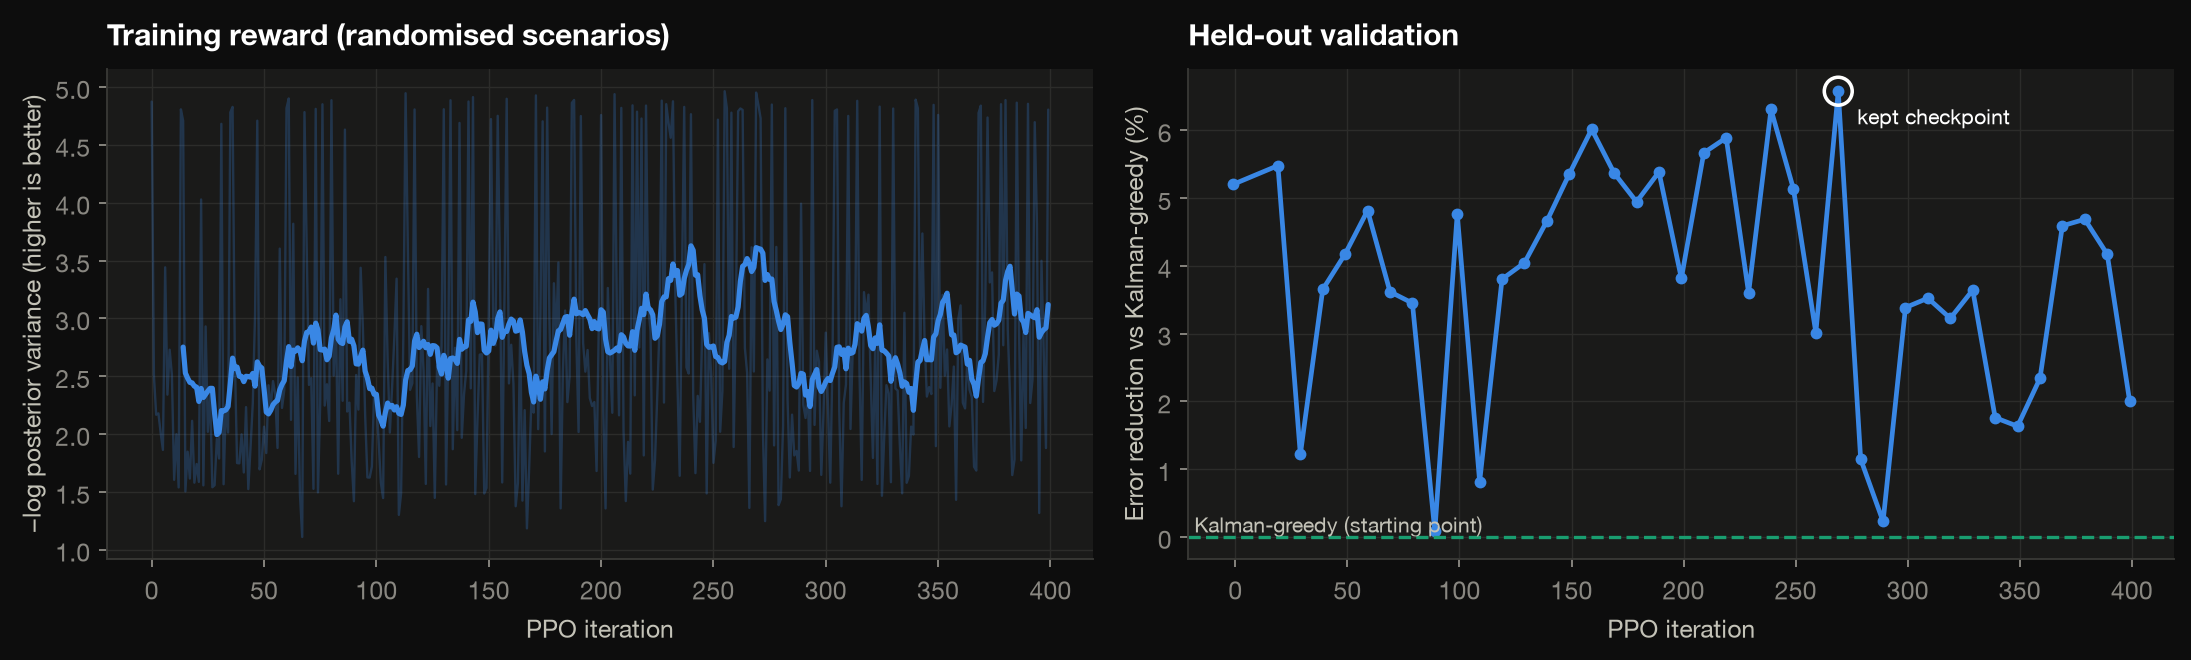
\includegraphics[width=\textwidth]{training.png}
\caption{Left: training reward. Right: validation improvement over Kalman-greedy.}\end{figure}

\textbf{Left.} Reward per PPO iteration (higher is better). It is noisy by design: each iteration uses a different
random network (size, capacity, correlation), so rewards differ a lot between iterations; the thick line is the
moving average, which trends upward.

\textbf{Right.} Held-out validation: how much lower the GNN's error is than Kalman-greedy's. The dashed line at 0 is
where training starts (the network \emph{is} Kalman-greedy at initialisation). It stays above 0 throughout and peaks at
+6.6\%; that checkpoint was kept.

\begin{saybox}
``Training starts exactly at the strongest classical scheduler, the dashed line, and every validation point after that
is better than it. We keep the best checkpoint, which is 6.6 percent better on held-out validation.''
\end{saybox}

%-------------------------------------------------------------------------------
\subsection{Figure: decision time}
\begin{figure}[H]\centering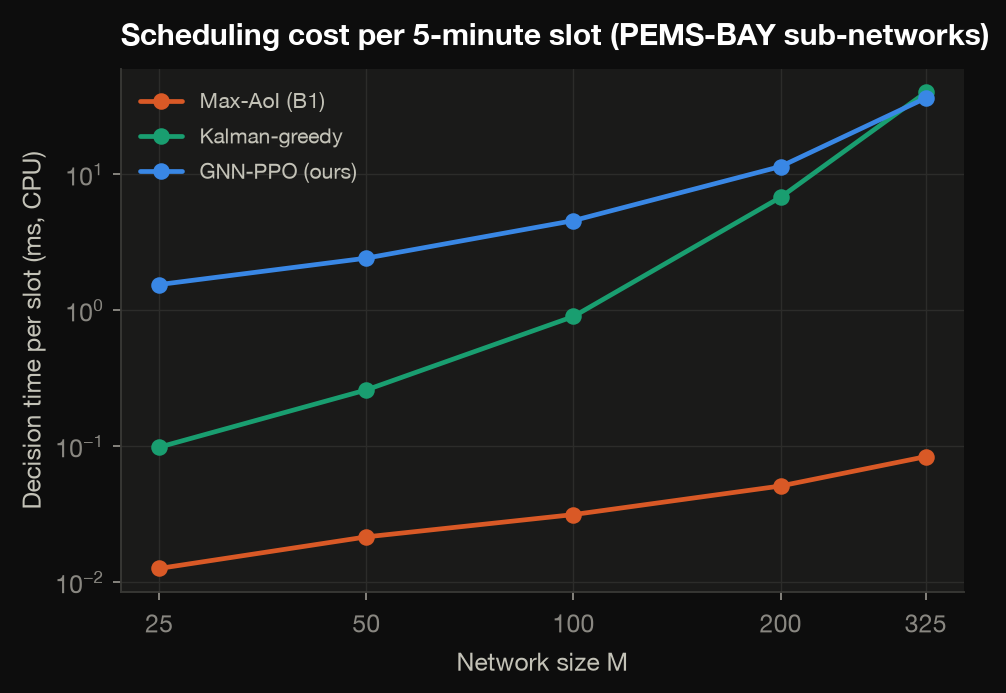
\includegraphics[width=0.6\textwidth]{decision_time.png}
\caption{Time to make one scheduling decision on a CPU, PEMS-BAY sub-networks (log scale).}\end{figure}

Max-AoI is almost free (under 0.1\,ms). Kalman-greedy grows steeply with size (0.1\,ms at 25 sensors to about 42\,ms at
325) because every pick updates the full covariance. The GNN costs 1.5\,ms at 25 sensors and about 37\,ms at 325, similar
to Kalman-greedy at full size. Either way, a decision takes less than a tenth of a second against a 300-second slot.

\begin{saybox}
``Even for 325 sensors a decision takes about 37 milliseconds on a laptop CPU, while a slot lasts 5 minutes, so the
scheduler easily runs in real time.''
\end{saybox}

%-------------------------------------------------------------------------------
\subsection{The live demo}
\begin{figure}[H]\centering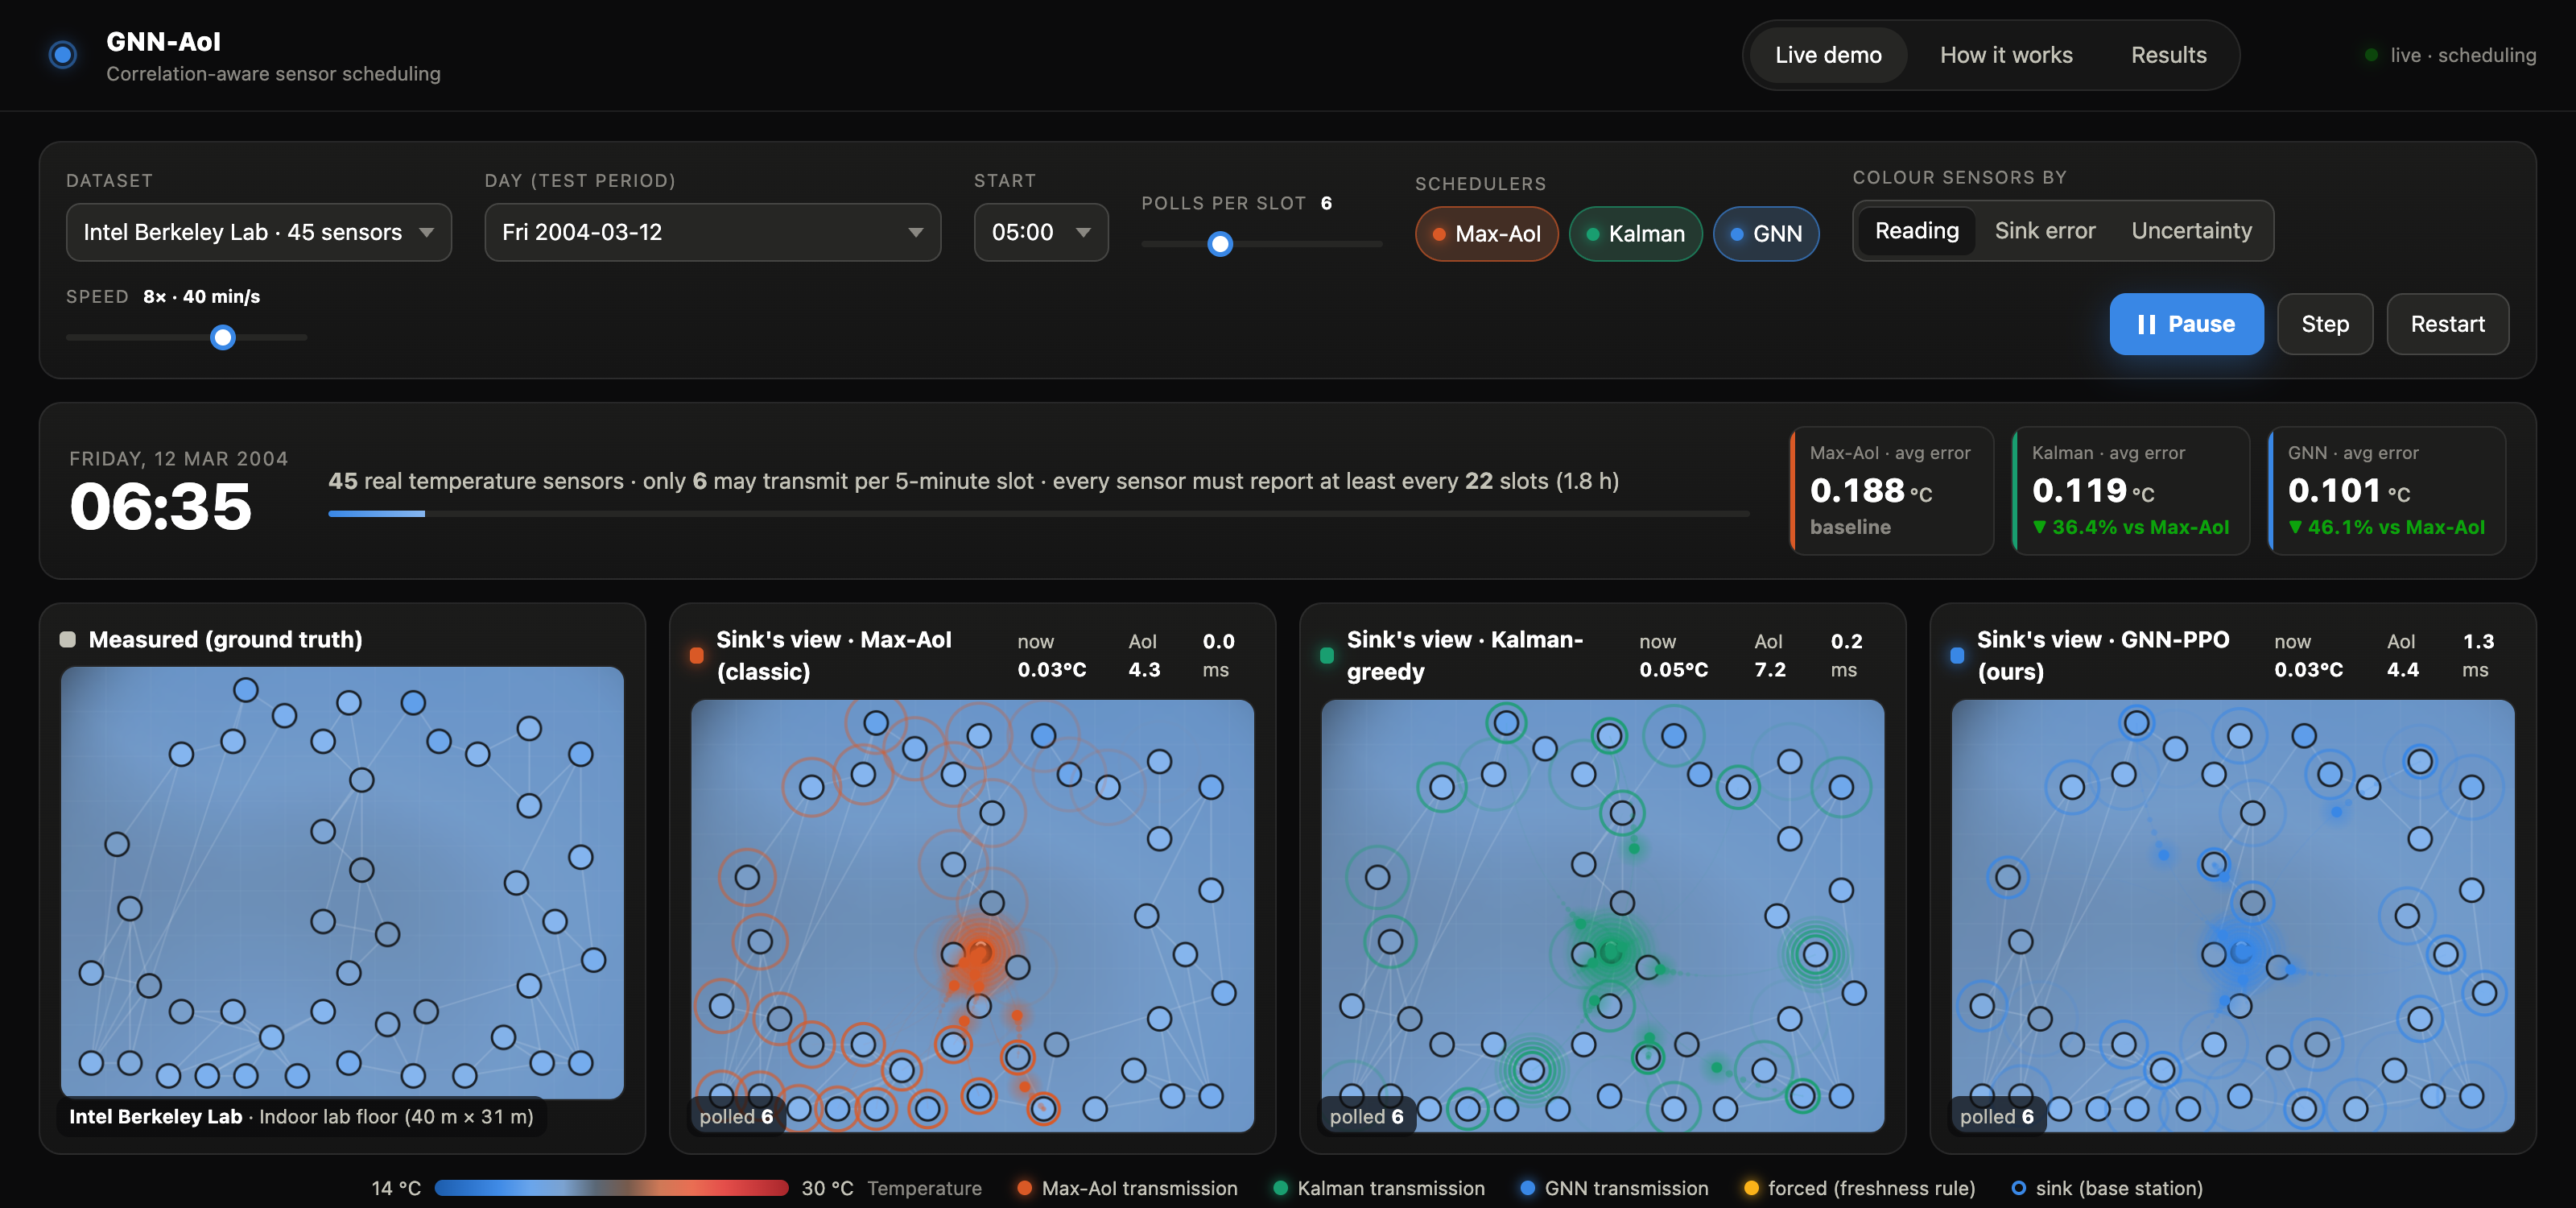
\includegraphics[width=\textwidth]{live_demo.png}
\caption{Live demo at \texttt{localhost:8000}, Intel Lab, Friday 12 March 2004, 06:35.}\end{figure}

\textbf{What each part shows.}
\begin{itemize}
  \item \textbf{Top controls}: dataset, test day, start hour, polls per slot, which schedulers to compare, how to colour
        sensors (reading, sink error, uncertainty), speed, play/step/restart.
  \item \textbf{Clock bar}: the real date and time being replayed and the running average error of each scheduler (here
        after 20 slots: Max-AoI 0.188\,$^\circ$C, Kalman 0.119\,$^\circ$C, GNN 0.101\,$^\circ$C, 46\% below Max-AoI).
  \item \textbf{Maps}: the measured floor, then each scheduler's view. Rings = sensors transmitting in this slot;
        a yellow ring = forced by the freshness rule.
  \item \textbf{Bottom}: error over time, ``Why these sensors?'' (the GNN's probability of picking each sensor first),
        and a transmission log listing which sensors each scheduler polled in each slot.
\end{itemize}

\begin{saybox}
``This is a real day from the test period, never used in training, replayed five minutes at a time. All three
schedulers see exactly the same readings. You can watch which six sensors each one polls, why the GNN chose them, and
how each base station's picture of the lab drifts from reality.''
\end{saybox}

\subsection{Comparison with recent literature}
\begin{center}
\small
\begin{tabularx}{\textwidth}{@{}p{3cm}XX@{}}
\toprule
\textbf{Work} & \textbf{Reported in their own setting} & \textbf{Same type of method on our real data} \\
\midrule
Ramakanth \emph{et al.}\ \cite{2} (base paper); Kadota \emph{et al.}\ \cite{16} & AoI-based scheduling within a constant factor of optimal & GNN lowers error 20\% (Intel) and 2.4\% (PEMS-BAY) vs.\ Max-AoI; wins 10/10 and 15/15 windows \\
Chen \emph{et al.}\ \cite{8} & Structure-enhanced DRL: 10--25\% lower MSE than benchmark DRL & GNN: 25.8\% (Intel) and 13.4\% (PEMS-BAY) lower MSE than Kalman-greedy \\
Krause \emph{et al.}\ \cite{19} & Greedy variance reduction is near-optimal per step & GNN beats it on 73\% of synthetic layouts, and beats it with the true covariance on 70\% \\
Reyhan \& Coleri \cite{9}; Farag \emph{et al.}\ \cite{7} & AoI limits met in probability & Hard bound, zero violations; greedy without a bound starves 18/50 sensors \\
\bottomrule
\end{tabularx}
\end{center}
The middle column comes from the cited papers' own setups and is not directly comparable; the right column re-runs that
class of method on our data under identical conditions.

\begin{saybox}[If the faculty asks: ``How do you compare with existing work?'']
``We cannot run their exact code on our data, so we re-implemented the type of method each paper uses: AoI-based
scheduling from our base paper and greedy uncertainty reduction from sensor-selection work. Under identical conditions,
on the same real test days, our scheduler beats both. Their own reported numbers are in a separate column so nobody
confuses the two.''
\end{saybox}
